\documentclass[oneside]{article}%You can define the type of paper here.
%%Useful packages that I commonly use.
%\usepackage[numbers]{natbib}%Bibliography package (help at http://merkel.zoneo.net/Latex/natbib.php).
%\usepackage{url}%Package to highlight url.
\usepackage{mathpazo}%Sets font to be math pazo.
\usepackage{alltt}%Allows the use of verbatim (good for printing out code).
%\usepackage{graphicx}%Used to import images.
\usepackage{amsmath, amssymb, amscd}%Contains the AMS expanded math symbols library.
\usepackage[explicit]{titlesec} %To remove section title in headers
%%For those who want smaller margins, you can use this:
\usepackage[top=1in, bottom=1in, left=1in, right=1in]{geometry}
\usepackage{fancyhdr} %%For headers/footers
%\usepackage{savetrees} %%Removes white space
\pagestyle{fancy} %%For fancy headers
\usepackage{tocloft}
\renewcommand{\cftsecleader}{\cftdotfill{\cftdotsep}}
\usepackage{pdfpages}
\usepackage{graphicx} %for including graphics and figures
\usepackage{enumerate} %for custom enumerations
\usepackage{caption} %for captions outside of floats
\usepackage{chemarr} %for using xrightleftharpoons for chemical reactions
\usepackage{multirow} % for using a table label that is multiple rows in size

\fancyhf{} %removes page enumeration from center middle of footer

\def\undertilde#1{\mathord{\vtop{\ialign{##\crcr
   $\hfil\displaystyle{#1}\hfil$\crcr\noalign{\kern1.5pt\nointerlineskip}
   $\hfil\tilde{}\hfil$\crcr\noalign{\kern1.5pt}}}}}


%for an approximate proportion symbol:
\def\approxprop{%
  \def\p{%
    \setbox0=\vbox{\hbox{$\propto$}}%
    \ht0=0.6ex \box0 }%
  \def\s{%
    \vbox{\hbox{$\sim$}}%
  }%
  \mathrel{\raisebox{0.7ex}{%
      \mbox{$\underset{\s}{\p}$}%
    }}%
}

\begin{document}
%% Top needs  to say "UNIVERSITY OF MONTANA: COMPUTER SCIENCE DEPARTMENT"
%%Title
\fancyhead[L]{CSCI 576 - HUMAN-COMPUTER INTERACTION} %%Header
\fancyhead[R]{\thepage} %Page enumeration
\fancyfoot[L]{BLAIR GEMMER - UNIVERSITY OF MONTANA: COMPUTER SCIENCE DEPARTMENT} %Footer
\rhead{}
\fancyhead[R]{\thepage} %Page enumeration
\renewcommand{\footrulewidth}{1pt}

%Fix headers on Table of Contents and List of Figures:
\fancypagestyle{plain}{
\fancyhead{}
\fancyfoot{}
\fancyhead[L]{CSCI 576 - HUMAN-COMPUTER INTERACTION} %%Header
\fancyfoot[L]{BLAIR GEMMER - UNIVERSITY OF MONTANA: COMPUTER SCIENCE DEPARTMENT} %Footer
\rhead{}
\renewcommand{\footrulewidth}{1pt}
}

\title{Zombie Tower Defense \\
	Project 1}
\author{Blair Gemmer}
\maketitle

\newcommand*\Hide{%
\titleformat{\chapter}[display]
  {}{}{0pt}{\Huge}
\titleformat{\part}
  {}{}{0pt}{}
}

\newpage
\subsection*{Description:}
\

The game will be similar to other desktop tower defense games in that the player
will be able to place “towers” on a map and the towers will fire at the enemy until the enemy is
destroyed. The main differences will be that the enemies will all be zombies or zombie-related
(such as zombie dogs or giant zombies), the towers will be zombie-survivors, and the towers
can be upgraded by giving the survivors different weapons. There will be a persistent leveling
system which will allow upgrades and a gold system to buy guns, more survivors, and better
armor/upgrades.\\

This game will be built for the android operating system, specifically 2.3+
(Gingerbread+).

\subsection*{Users:}
\

The users of this system will be all ages. They will include people who enjoy simple flash
games, desktop tower defense games, and zombie killing games.

\subsection*{Usability Requirements:}
\

The game will need to be fun, be easy to learn with simple addictive
game play, easy to put down and return to without interruption, have persistent in-game
achievements and upgrades, and be challenging.

\subsection*{Functional Requirements:}


\begin{enumerate}[*]

	\item User should be able to navigate a simple menu before entering the game.
	\item User should be able to choose the number of players for a new game.
	\item User should be able to choose from various options or settings before entering the game.
	\item User should be able to continue a game from a previous save point before entering the game.
	\item User should be able to choose a specific mission before entering the game
	\item User should be able to hit pause/play with a single button while in game.
	\item User should be able to choose options/settings within the game.
	\item User should be able to see his/her level inside the game.
	\item User should be able to see their current gold inside the game.
	\item User should be able to buy or upgrade their characters while playing the game.
	\item User should be able to see the number of zombies killed, survivors that died, and the total
amount of gold earned at the end of each round in a scoreboard-type fashion.
	\item User should be able to save game state and return to the same game state without
interruption.
	\item User should be able to take phone calls or check messages without interrupting game state.
	\item User should be able to engage different types of enemies.
	\item User should be able to create a custom map or choose from a list of available maps.
	\item User should be able to open new maps / levels by finishing the previous map / level.
	\item User should be able to upgrade survivor’s guns or armor with gold earned.
	\item User should be able to buy new or replacement survivors using gold earned. (“dead” survivors become zombies?)
	\item User should be able to earn achievements by leveling up over time. These achievements
should include new survivor types, new survivor weapons, and skill trees for defensive and
offensive help.
	\item User should be able to unlock a variety of weapons, such as melee weapons (swords,
machete, chainsaw, baseball bat, crowbar, etc), pistols (revolvers, semi-auto, full-auto),
shotguns (pump-action, semi-auto, full-auto), machine gun, machine gun sentries, rocket
launcher, rocket launcher sentries, grenade launcher, grenade launcher sentries, flamethrower,
and many more to come.
	\item User should be able to unlock a variety of upgrades, such as armor, larger ammo clips, faster
reload, better aim, etc
	\item User should be able to choose some premium services, such as changing uniforms of
survivors or avatar, access to new maps, multi-player mode, custom map editor, access to new
weapons, etc.
	\item User should be able to change options for muting sound effects and background sounds
\end{enumerate}

\subsection*{Sketches:}
\

\begin{enumerate}
	\item Menu UI
	\item In-Game UI
	\item Map Editor
	\item Character Editor
	\item Score UI
	\item Store UI
\end{enumerate}

\subsection*{Use Cases:}
\

\begin{enumerate}
	\item Choosing a mission
	\item Choosing a previously saved game
	\item Upgrading a weapon or stats
	\item Scoreboard
	\item Creating a map
	\item Buying a new survivor or turret
	\item Playing the game
\end{enumerate}
%for creating a table (notice the multicolumn and multirow commands also for formatting the labels)
%\begin{center}
%	\begin{tabular}{| l | l | l | l | l |}
%		\hline
%		\multirow{3}{*}{Day \#}  & \multicolumn{4}{c}{Mean density}\vline\\
%		\cline{2-5}
%		& \multicolumn{2}{c}{In isolation} \vline& \multicolumn{2}{c}{In competition}\vline\\
%		\cline{2-5}
%		& \textit{P. aurelia} & \textit{P. caudatum} & \textit{P. aurelia} & \textit{P. caudatum}\\
%		\hline
%		0 & 2 & 2 & 2 & 2\\
%		\hline
%		1 & | & | & | & |\\
%		\hline
%		2 & a & b & c & d\\
%		\hline
%	\end{tabular}
%	\captionof{table}{Summary of the cases shown in Figure 3.}
%\end{center}

%for creating a vector or matrix, floating to the left:
%$f(x) =$ \( \left[ \begin{array}{ccc}
%a&b&c\\
%d&e&f
%\end{array} \right]\) 
%
%%for creating a vector or matrix, floating to the right:
%$f(x) =$ \[ \left[ \begin{array}{ccc}
%a&b&c\\
%d&e&f
%\end{array} \right]\] 

%For creating an image with a caption:
%\begin{minipage}{\linewidth}
%		\makebox[\linewidth]{%
%		\centering
%		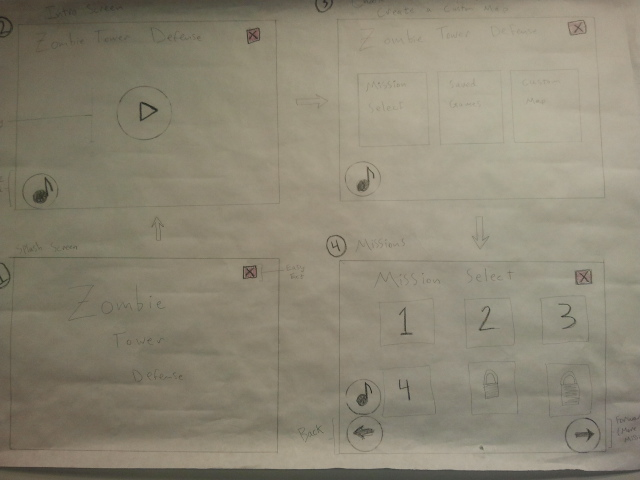
\includegraphics[scale=.1]{plots/problem242/1.jpg}}
%		\captionof{figure}{Plot of $a_n$ along time $n$, showing the oscillation between $a_{max}$ and $a_{min}$, }
%		\captionof*{figure}{where $a_{max} = $ toxicity of a drug and $a_{min} = $ effectual level of drug.}
%		\end{minipage}\\


\end{document}